\documentclass[11pt,letterpaper]{article}
\usepackage{xcolor}
\usepackage{textcomp,marvosym}
\usepackage{amsmath,amssymb}
\usepackage[left]{lineno}
\usepackage{changepage}
\usepackage{rotating}
\usepackage{natbib}
\usepackage{setspace}
\usepackage{fancyhdr}
\usepackage{graphicx}
\usepackage{sidecap}
\usepackage{pdfpages}
\usepackage{longtable}
\usepackage{url}
\usepackage[aboveskip=1pt,labelfont=bf,labelsep=period,justification=raggedright,singlelinecheck=off]{caption}
%\doublespacing

\raggedright
\textwidth = 6.5 in
\textheight = 8.5 in
\oddsidemargin = 0.0 in
\evensidemargin = 0.0 in
\topmargin = -0.5 in
\headheight = 0.0 in
\headsep = 0.5 in
\parskip = 0.0 in
\parindent = 0.2 in

\begin{document}
\renewcommand{\thefigure}{S\arabic{figure}}
\renewcommand{\thetable}{S\arabic{table}}
\subsection*{Supporting Information for ``Bayesian paleomagnetic Euler pole inversion for paleogeographic reconstruction and analysis"}

\begin{figure}[h!]
\noindent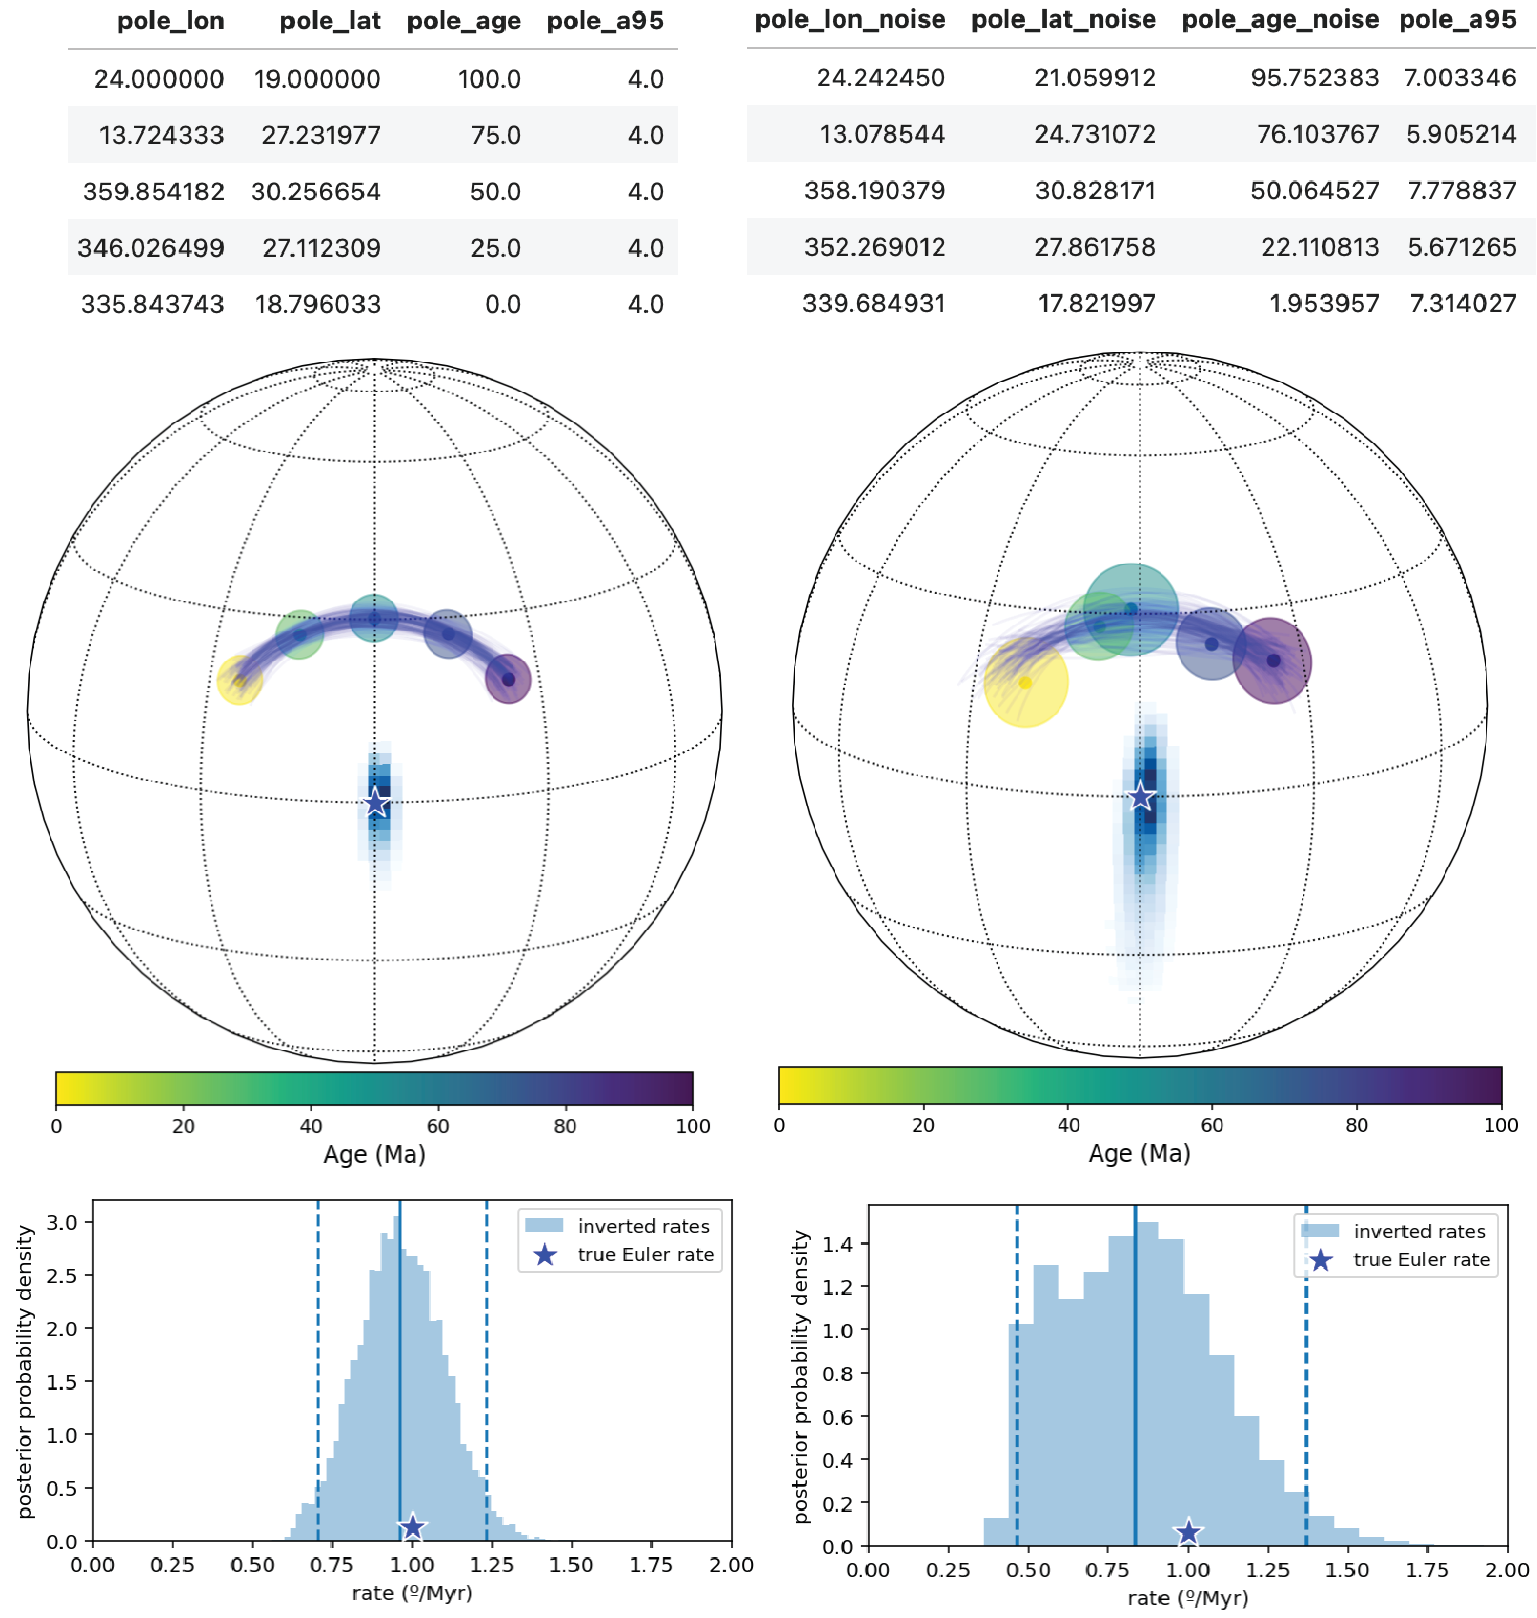
\includegraphics[width=6 in]{SI_fig_synthetic_noise.pdf}
\caption{The left panel is the inversion for five paleomagnetic poles are generated during a net $100^\circ$ rotation about an Euler pole at $00^\circ$N, $000^\circ$E over 100 Myr that is shown in Figure 4 of the main text. The right panel is an example where noise is introduced in terms of the position of the synthetic poles and their age. The inversion is able to recover the true Euler position and rate within the credible intervals of the posterior distributions although these credible intervals are larger.}
\label{pdffiguresample}
\end{figure}


\begin{figure}[h!]
\noindent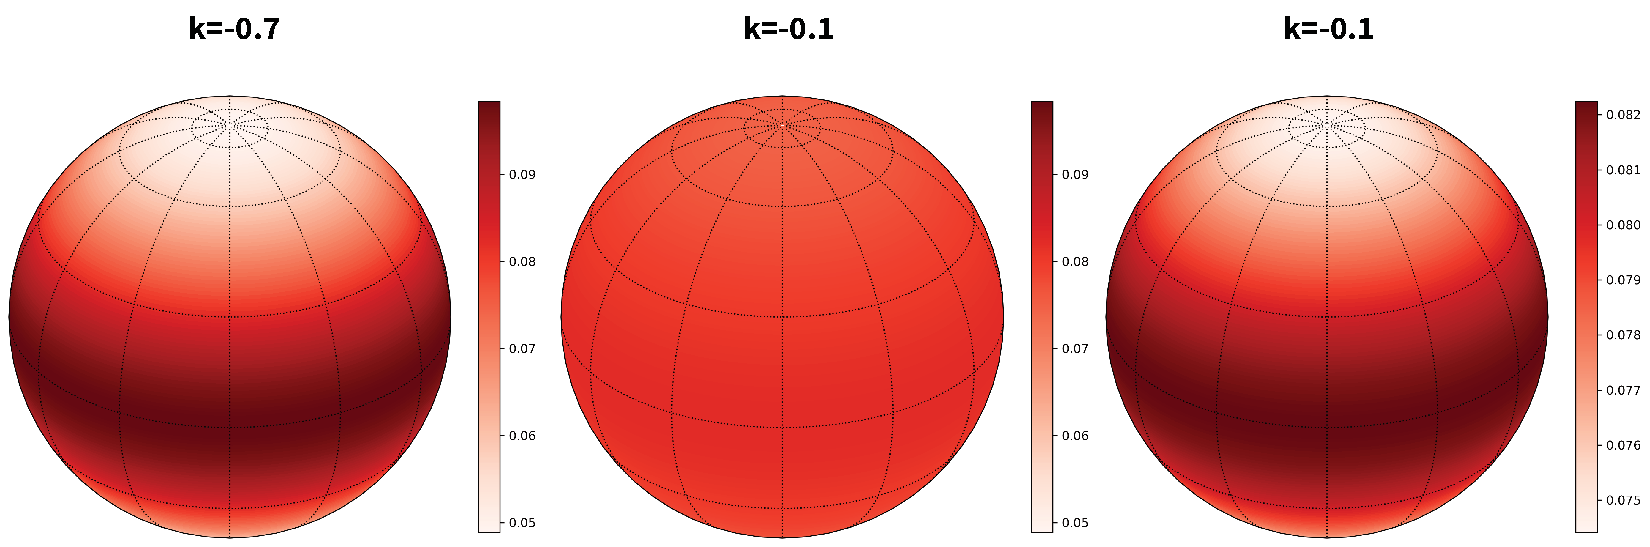
\includegraphics[width=\textwidth]{SI_fig_Euler_prior.pdf}
\caption{The probability distribution associated with Watson girdle distributions comparing that arising from the Euler pole prior analysis in Figure 3 that yielded $\kappa_w=-0.7$ and that of $\kappa_w=-0.1$ that was used for a more quickly informed prior associated with inversions.  $\kappa_w=-0.1$ is shown with the same color scale as $\kappa_w=-0.7$ in the middle panel and also with a color scale that is scaled to the 2 and 98 percentile of the density in the right panel.}
\label{pdffiguresample}
\end{figure}
\end{document}

% %\clearpage

% %Delete all unused file types below. Copy/paste for multiples of each file type as needed.
% \noindent\textbf{Text S1.}
% %Type or paste text here. This should be additional explanatory text, such as: extended descriptions of results, full details of models, extended lists of acknowledgements etc.  It should not be additional discussion, analysis, interpretation or critique. It should not be an additional scientific experiment or paper.
% %
% %Repeat for any additional Supporting Text

% %%Enter Data Set, Movie, and Audio captions here
% %%EXAMPLE CAPTIONS

% \noindent\textbf{Data Set S1.} %Type or paste caption here.
% %upload your dataset(s) to AGU's journal submission site and select "Supporting Information (SI)" as the file type. Following naming %convention: ds01.

% %Repeat for any additional Supporting data sets

% \noindent\textbf{Movie S1.} %Type or paste caption here.
% %upload your movie(s) to AGU's journal submission site and select, "Supporting Information %(SI)" as the file type. Following naming convention: ms01.

% %Repeat any additional Supporting movies

% \noindent\textbf{Audio S1.} %Type or paste caption here.
% %upload your audio file(s) to AGU's journal submission site and select "Supporting Information %(SI)" as the file type. Following naming convention: auds01.


% %Repeat for any additional Supporting audio files

% %%% End of body of article:
% %%%%%%%%%%%%%%%%%%%%%%%%%%%%%%%%%%%%%%%%%%%%%%%%%%%%%%%%%%%%%%%%
% %
% % Optional Notation section goes here
% %
% % Notation -- End each entry with a period.
% % \begin{notation}
% % Term & definition.\\
% % Second term & second definition.\\
% % \end{notation}
% %%%%%%%%%%%%%%%%%%%%%%%%%%%%%%%%%%%%%%%%%%%%%%%%%%%%%%%%%%%%%%%%


% %% ------------------------------------------------------------------------ %%
% %%  REFERENCE LIST AND TEXT CITATIONS

% %%%%%%%%%%%%%%%%%%%%%%%%%%%%%%%%%%%%%%%%%%%%%%%
% % 
% %
% % \bibliography{<name of your .bib file>} do not specify file extension
% %
% % no need to specify bibliographystyle
% %
% % Note that ALL references in this supporting information file must also be referenced in the primary manuscript
% %
% %%%%%%%%%%%%%%%%%%%%%%%%%%%%%%%%%%%%%%%%%%%%%%%
% % if you get an error about newblock being undefined, uncomment this line:
% %\newcommand{\newblock}{}

% % \bibliography{ uncomment this line and enter the name of your bibtex file here } 




% %Reference citation instructions and examples:
% %
% % Please use ONLY \cite and \citeA for reference citations.
% % \cite for parenthetical references
% % ...as shown in recent studies (Simpson et al., 2019)
% % \citeA for in-text citations
% % ...Simpson et al (2019) have shown...
% % DO NOT use other cite commands (e.g., \citet, \citep, \citeyear, \nocite, \citealp, etc.).
% %
% %
% %...as shown by \citeA{jskilby}.
% %...as shown by \citeA{lewin76}, \citeA{carson86}, \citeA{bartoldy02}, and \citeA{rinaldi03}.
% %...has been shown \cite<e.g.,>{jskilbye}.
% %...has been shown \cite{lewin76,carson86,bartoldy02,rinaldi03}.
% %...has been shown \cite{lewin76,carson86,bartoldy02,rinaldi03}.
% %
% % apacite uses < > for prenotes, not [ ]
% % DO NOT use other cite commands (e.g., \citet, \citep, \citeyear, \nocite, \citealp, etc.).
% %

% %% ------------------------------------------------------------------------ %%
% %
% %  END ARTICLE
% %
% %% ------------------------------------------------------------------------ %%
% \end{article}
% \clearpage

% % Copy/paste for multiples of each file type as needed.

% % enter figures and tables below here: %%%%%%%
% %
% %
% %
% %
% % EXAMPLE FIGURES
% % ---------------
% % If you get an error about an unknown bounding box, try specifying the width and height of the figure with the natwidth and natheight options.
% % \begin{figure}
% %\setfigurenum{S1} %%You can change number for each figure if you want, not required. "S" prepended automatically.
% % \noindent\includegraphics[natwidth=800px,natheight=600px]{samplefigure.eps}
% %\caption{caption}
% %\label{epsfiguresample}
% %\end{figure}
% %
% %
% % Giving latex a width will help it to scale the figure properly. A simple trick is to use \textwidth. Try this if large figures run off the side of the page.
% % \begin{figure}
% % \noindent\includegraphics[width=\textwidth]{anothersample.png}
% %\caption{caption}
% %\label{pngfiguresample}
% %\end{figure}
% %
% %
% %\begin{figure}
% %\noindent\includegraphics[width=\textwidth]{athirdsample.pdf}
% %\caption{A pdf test figure}
% %\label{pdffiguresample}
% %\end{figure}
% %
% % PDFLatex does not seem to be able to process EPS figures. You may want to try the epstopdf package.
% %
% %
% % ---------------
% % EXAMPLE TABLE
% %
% %\begin{table}
% %\settablenum{S1} %%Change number for each table
% %\caption{Time of the Transition Between Phase 1 and Phase 2\tablenotemark{a}}
% %\centering
% %\begin{tabular}{l c}
% %\hline
% % Run  & Time (min)  \\
% %\hline
% %  $l1$  & 260   \\
% %  $l2$  & 300   \\
% %  $l3$  & 340   \\
% %  $h1$  & 270   \\
% %  $h2$  & 250   \\
% %  $h3$  & 380   \\
% %  $r1$  & 370   \\
% %  $r2$  & 390   \\
% %\hline
% %\end{tabular}
% %\tablenotetext{a}{Footnote text here.}
% %\end{table}
% % ---------------
% %
% % EXAMPLE LARGE TABLE (UPLOADED SEPARATELY)
% %\begin{table}
% %\settablenum{S1} %%Change number for each table
% %\caption{Time of the Transition Between Phase 1 and Phase 2\tablenotemark{a}}
% %\end{table}


\end{document}

%%%%%%%%%%%%%%%%%%%%%%%%%%%%%%%%%%%%%%%%%%%%%%%%%%%%%%%%%%%%%%%

More Information and Advice:

%% ------------------------------------------------------------------------ %%
%
%  SECTION HEADS
%
%% ------------------------------------------------------------------------ %%

% Capitalize the first letter of each word (except for
% prepositions, conjunctions, and articles that are
% three or fewer letters).

% AGU follows standard outline style; therefore, there cannot be a section 1 without
% a section 2, or a section 2.3.1 without a section 2.3.2.
% Please make sure your section numbers are balanced.
% ---------------
% Level 1 head
%
% Use the \section{} command to identify level 1 heads;
% type the appropriate head wording between the curly
% brackets, as shown below.
%
%An example:
%\section{Level 1 Head: Introduction}
%
% ---------------
% Level 2 head
%
% Use the \subsection{} command to identify level 2 heads.
%An example:
%\subsection{Level 2 Head}
%
% ---------------
% Level 3 head
%
% Use the \subsubsection{} command to identify level 3 heads
%An example:
%\subsubsection{Level 3 Head}
%
%---------------
% Level 4 head
%
% Use the \subsubsubsection{} command to identify level 3 heads
% An example:
%\subsubsubsection{Level 4 Head} An example.
%
%% ------------------------------------------------------------------------ %%
%
%  IN-TEXT LISTS
%
%% ------------------------------------------------------------------------ %%
%
% Do not use bulleted lists; enumerated lists are okay.
% \begin{enumerate}
% \item
% \item
% \item
% \end{enumerate}
%
%% ------------------------------------------------------------------------ %%
%
%  EQUATIONS
%
%% ------------------------------------------------------------------------ %%

% Single-line equations are centered.
% Equation arrays will appear left-aligned.

Math coded inside display math mode \[ ...\]
 will not be numbered, e.g.,:
 \[ x^2=y^2 + z^2\]

 Math coded inside \begin{equation} and \end{equation} will
 be automatically numbered, e.g.,:
 \begin{equation}
 x^2=y^2 + z^2
 \end{equation}

% IF YOU HAVE MULTI-LINE EQUATIONS, PLEASE
% BREAK THE EQUATIONS INTO TWO OR MORE LINES
% OF SINGLE COLUMN WIDTH (20 pc, 8.3 cm)
% using double backslashes (\\).

% To create multiline equations, use the
% \begin{eqnarray} and \end{eqnarray} environment
% as demonstrated below.
\begin{eqnarray}
  x_{1} & = & (x - x_{0}) \cos \Theta \nonumber \\
        && + (y - y_{0}) \sin \Theta  \nonumber \\
  y_{1} & = & -(x - x_{0}) \sin \Theta \nonumber \\
        && + (y - y_{0}) \cos \Theta.
\end{eqnarray}

%If you don't want an equation number, use the star form:
%\begin{eqnarray*}...\end{eqnarray*}

% Break each line at a sign of operation
% (+, -, etc.) if possible, with the sign of operation
% on the new line.

% Indent second and subsequent lines to align with
% the first character following the equal sign on the
% first line.

% Use an \hspace{} command to insert horizontal space
% into your equation if necessary. Place an appropriate
% unit of measure between the curly braces, e.g.
% \hspace{1in}; you may have to experiment to achieve
% the correct amount of space.


%% ------------------------------------------------------------------------ %%
%
%  EQUATION NUMBERING: COUNTER
%
%% ------------------------------------------------------------------------ %%

% You may change equation numbering by resetting
% the equation counter or by explicitly numbering
% an equation.

% To explicitly number an equation, type \eqnum{}
% (with the desired number between the brackets)
% after the \begin{equation} or \begin{eqnarray}
% command.  The \eqnum{} command will affect only
% the equation it appears with; LaTeX will number
% any equations appearing later in the manuscript
% according to the equation counter.
%

% If you have a multiline equation that needs only
% one equation number, use a \nonumber command in
% front of the double backslashes (\\) as shown in
% the multiline equation above.

%% ------------------------------------------------------------------------ %%
%
%  SIDEWAYS FIGURE AND TABLE EXAMPLES
%
%% ------------------------------------------------------------------------ %%
%
% For tables and figures, add \usepackage{rotating} to the paper and add the rotating.sty file to the folder.
% AGU prefers the use of {sidewaystable} over {landscapetable} as it causes fewer problems.
%
% \begin{sidewaysfigure}
% \includegraphics[width=20pc]{samplefigure.eps}
% \caption{caption here}
% \label{label_here}
% \end{sidewaysfigure}
%
%
%
% \begin{sidewaystable}
% \caption{}
% \begin{tabular}
% Table layout here.
% \end{tabular}
% \end{sidewaystable}
%
%

